\section{Dirichlet belief networks}
As can be seen from the above, the prior distribution of topics and word matrices should obey Dirichlet distribution, which is an effective assumption, but it also brings many limitations. Recently,people introduce different generative models based on Latent Dirichle Model
\subsection{Research on Topic Distribution}

The LDA model assumes that the topics are independent of each other, however, this assumption
It is very inconsistent with the actual data set. To overcome this defect, in 2006 Blei proposes a related topic model called Correlated Topic Model,
CTM\cite{corr}, the model extracts the topic from the Logistic Normal distribution, succeddfully overcoming the disadvantage that LDA model cannot extract relatation of  information between documents. This model mentioned
above have been successfully applied in extracting scientific subjects and image extraction.

Another well-known research on topic-distribution is Hierarchical Dirichlet processes\cite{Teh}. Based on the deformation of Dirichlet Process, HDP is A non-parametric Bayesian model that can automatically train the most suitable from the document set appropriate number of topics $K$. Nonparametric characteristics of HDP through Dirichlet process solve the problem of selecting the number of topics in LDA model, and the experiment confirms  that the optimal number of topics selected by HDP model is equal to the optimal number of topics selected based on perplexity.

LDA model assumes that topic of each word is subject to multinomial distribution and the document is converted into count  matrix by Bag of Word model.Poisson Factor Analysis \cite{han}  introduces poisson distribution to generate the words of document. The total count of word will be assign different latent topic.
\[
  x_{pi} = \sum_{k=1}^{K} x_{pik}
\]
\[
  x_{pik} \sim Pois(\gamma_{pk}\theta_{ki})
\]
and topic-distribution is subject to gamma distribution:
\[
  \theta_{ki} \sim Gamma(r_k,\frac{p_k}{1-p_k})
\]

\subsection{Introduction of DIRBN}
Compared to considerable researchs  topic model,the word model has not been fully studied and The Dirichlet Belief Network (DBN)\cite{Zhao} introduces a deep generative model where each layer is weighted by sets of  topics.

Different from single layer dirichlet,DirBN model proposed a multi-layer Dirchlet layer generative process on word-distribution.The latent distributions in each layer of DBN are generated as Dirichlet
random variables and can thus be interpreted as categorical
distributions.Then  the hidden units are connected with gamma-distributed weights.

\begin{figure}[htbp]
% \centering % 图片居中
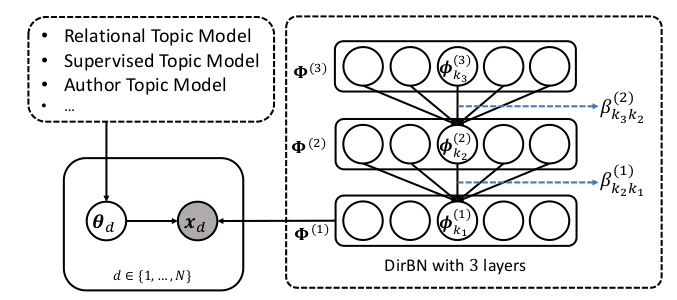
\includegraphics[width = 13cm]{dirbn.png}
\caption{DirBN Model}
\label{fig:DirBN Model}
\end{figure}

In comparison to existing deep generative models,DirBN have better Interpretability on topics annd higher modelling accuracy.However,the current formulation of DBN odel suffers from decay during information passing.

DBN’s deep architecture is currently limited to
only a few layers. In order to obtain efficient Gibbs sam-
pling, DBN back-propagates the observed information from
the output layer to each hidden layer. The cost of the in-
formation back-propagation is that the information would
decay in a O(log) rate on passing through one layer to its
upper layer \cite{Zhou}. Therefore, little informa-
tion might be available after a few layer back-propagations
\subsection{Inference of DirBN}
The training of DirBN model introduce several data augmentation techniques in the inference of latent variables.
Given topic-doc matrix $\theta$ and topic-word matrix $\phi$we can sample the topic of each word ini each document.Then we get the topic-word count matrix $x_{k_1}^{(1)} = [x_{1k_1}^{(1)},\dots,x_{Vk_1}^{(1)}]$ which is also the input count vector of DirBN inference process.
The process of Inference involve two key parts:
\begin{enumerate}
  \item Propagating the input count vector from
Bottom to top.Due to the inconjugate property between these latent distri-butions, direct efficient Gibbs sampling over these random variables is difficult. Insteadchoose to first back propagates the observed counting information into each layer and then proceed forward variable Gibbs sampling.
\item updating latent parameters from top to bottom.After back propagatation of latent count,update the variables by conjugate posterior distribution.

\end{enumerate}
